\section{External versus heap and quicksort}

Using the results from previous tests we declared a winning strategy for external sorting - bufferedStream with a buffer size of 1024 and a d value of 32. We then ran this setup for several values of N. The same N values were used for a standard quicksort and heapsort implementation.

Heapsort's time grew extremely fast as soon as swap space had to be used for large values of N so eventually we decided to stop these tests as they would simply require to much time to complete. Heapsort is often hailed as having a worst case that is better than Quicksort, however this only happens for internal sorting as the required I/Os to maintain the heap far outweigh other time constrains.

Next we looked at Quicksort compared to external merge sort. We expected Quicksort to perform a lot better than Heapsort, and it did, however we had also expected the difference between quicksort and the external sort to be more in favour of external sorting as N gew. As can be see from the graph this was not always the case.

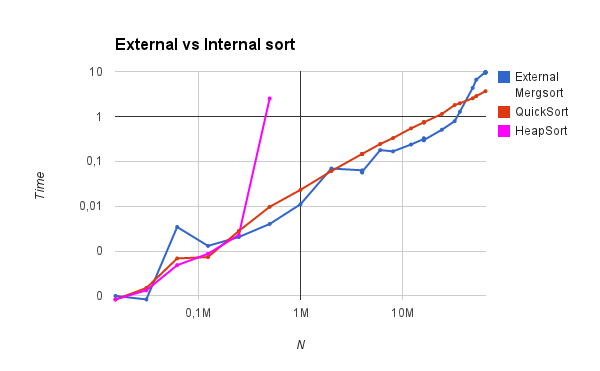
\includegraphics[width=90mm]{parts/compare.png}

When the number of items to be sorted is low enough to fit into memory both heapsort and quicksort performs better than External - remember our memory is limited to 1 mb during this experiments - however as soon as that value is exceed external sorting becomes a lot better than Heapsorting. Quicksort on the other hand increases in a logarithm fashion seemingly no matter how large N became. In fact quicksort becomes faster than the external merge sort for very large vaules - this was not as we had predicated! More tests would be required to find the exact reason for this, but we suspect it is in fact due to implementation details of our merge sorting. We use Vectors to keep track of the paths and streams which may end up giving us a unnecessary large overhead. Up untill this point our merge sorting does out perform Quicksort.